\documentclass[aspectratio=1610]{beamer}
\usetheme{Madrid}

\usepackage{amsmath}
\usepackage{graphicx}
\usepackage{amssymb}
\usepackage{listings}
\usepackage{booktabs}
\usepackage{multirow}
\usepackage{lmodern}
\usepackage{xcolor}
\usepackage{float}
\lstset{
  language=Python,
  rulesepcolor=\color{red!20!green!20!blue!20},
  keywordstyle=\color{blue!90}\bfseries,
  commentstyle=\color{red!10!green!70}\textit,
  basicstyle=\footnotesize,
  showstringspaces=true,
  stringstyle=\rmfamily\slshape\color[RGB]{128,0,0},
  breaklines=true,
  extendedchars=false,
  escapeinside=``,
  texcl=true
}

\lstset{breaklines}
\lstset{extendedchars=false}

\usepackage{textcomp}
\usepackage{pythonhighlight}
\usepackage[backend=bibtex,style=authoryear]{biblatex}
\addbibresource{reference.bib}

\usepackage{algorithm}
\usepackage{algorithmic}
\renewcommand{\algorithmicrequire}{\textbf{Input:}}
\renewcommand{\algorithmicensure}{\textbf{Output:}}

\usepackage{tikz}
\tikzstyle{startstop} = [rectangle, rounded corners, minimum width=3cm, minimum height=1cm,text centered, draw=black, fill=blue!30]
\tikzstyle{process} = [rectangle, minimum width=2cm, minimum height=1cm, text centered, draw=black, fill=brown!30]
\tikzstyle{arrow} = [thick,->,>=stealth]
\title[short]{long and long}
\author[Gcc]{Dingchao Gao}
\institute[ISCAS]{Institute of Software Chinese Academy of Sciences}

\begin{document}

\begin{frame}[plain]
  \titlepage
  %  Title page
\end{frame}
\begin{frame}[noframenumbering,allowframebreaks,t]
	\frametitle{references}
	\printbibliography
\end{frame}
\begin{frame}
  \begin{center}
    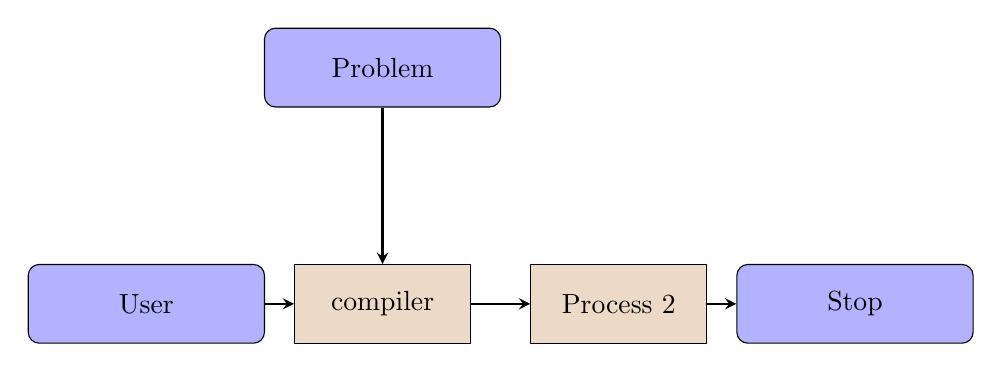
\begin{tikzpicture}[node distance=3cm, every node/.style={text width=2cm, align=center}]

      \node (start) [startstop] {User};
      \node (process1) [process, right of=start] {compiler};
      \node (problem) [startstop, above of = process1] {Problem};
      \node (process2) [process, right of=process1] {Process 2};
      \node (stop) [startstop, right of=process2] {Stop};
      \draw [arrow] (start) -- (process1);
      \draw [arrow] (problem) -- (process1);
      \draw [arrow] (process1) -- (process2);
      \draw [arrow] (process2) -- (stop);
      \end{tikzpicture}
  \end{center}
\end{frame}
\begin{frame}
\centering
\Huge{END\\Thank you}
\end{frame}
\end{document}